L'utilisation de lasers puissants dans un système expérimental doit être une des premières préoccupations de la personne responsable.

Dans le cadre de ce travail de bachelor, deux niveaux de protection ont été élaborés afin de garantir au mieux la sécurité du laser :

\begin{enumerate}
    \item Le premier niveau est mécanique et comprend deux mécanismes :
          \begin{itemize}
              \item La première est située à l'entrée du faisceau laser.
              \item La seconde est située vers le microscope, en fin de trajet du laser.
          \end{itemize}
    \item Le deuxième niveau est électrique et repose sur deux dispositifs :
          \begin{itemize}
              \item Le système intégré interlock du driver du laser va être modifié pour fonctionner avec les protections mécaniques.
              \item Un boitier contenant un bouton d'arrêt d'urgence ainsi qu'une clé de maintenance vont être apportés en plus dans le système interlock.
          \end{itemize}
\end{enumerate}

Les sections suivantes expliquent en détail les différents systèmes réalisés.

\section{Sécurité électrique}

Pour la sécurité au niveau électrique, le but va être d'ajouter aux protections mécaniques, des capteurs afin de déterminer quand une protection est ouverte.

Pour ajouter plus de sécurité, un arrêt d'urgence ainsi qu'une clé de maintenance vont être ajoutés. Ces deux capteurs, l'arrêt d'urgence ainsi que la clé de maintenance, vont être relié ensemble et connecté au interlock du driver du laser.

\newpage
\subsection{Interlock: Principe de fonctionnement}

\begin{minipage}[c]{0.6\textwidth}
    Le driver du laser intègre un système d'interlock, qui permet de, si le circuit électrique interlock est ouvert, désactiver l'alimentation du laser. Par défaut, un pont est soudé entre les pins 1 et 5, voir la Figure~\ref{No_interlock} ci-contre.
\end{minipage}\hfill
\begin{minipage}[c]{0.35\textwidth}
    \begin{figure}[H]
        \begin{center}
            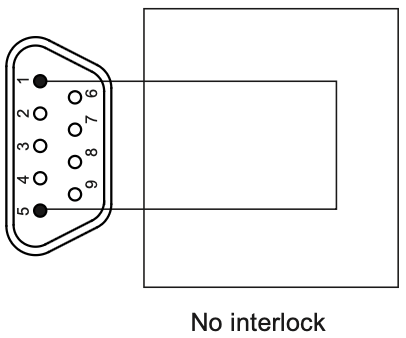
\includegraphics[width=0.8\textwidth]{assets/figures/Protections_laser/no_interlock.png}
        \end{center}
        \captionof{figure}{Schéma électrique sans interlock~\cite{LaserDriverKLD101}}
        \label{No_interlock}
    \end{figure}
\end{minipage}
\begin{minipage}[c]{0.6\textwidth}
    Le but étant d'ajouter un circuit électrique personalisé qui intègre l'interlock, de ce fait, le schéma suivant va être utilisé pour la conception du circuit électrique. Voir la Figure~\ref{Interlock_only}, ci-contre.
\end{minipage}\hfill
\begin{minipage}[c]{0.35\textwidth}
    \begin{figure}[H]
        \begin{center}
            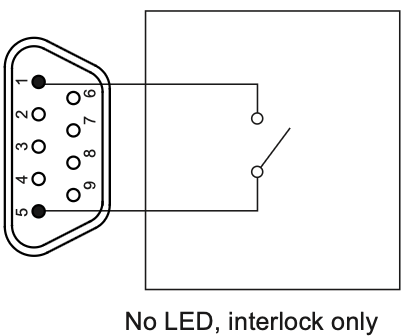
\includegraphics[width=0.8\textwidth]{assets/figures/Protections_laser/interlock_only.png}
        \end{center}
        \captionof{figure}{Schéma électrique avec interlock~\cite{LaserDriverKLD101}}
        \label{Interlock_only}
    \end{figure}
\end{minipage}

Ci-dessous, voir Figure\ref{schema_interlock_v1}, est la première version du schéma électrique complet pour l'interlock. Étant donné que le choix des capteurs n'est pas encore fait à ce stade, des fins de course ont été représentés de façon provisoire, afin d'avoir une première représentation fonctionnelle du système. L'arrêt d'urgence ainsi que la clé de maintenance vont être expliqué dans la section~\ref{subsec:arret_urgence_maintenance}.

\begin{figure}[H]
    \begin{center}
        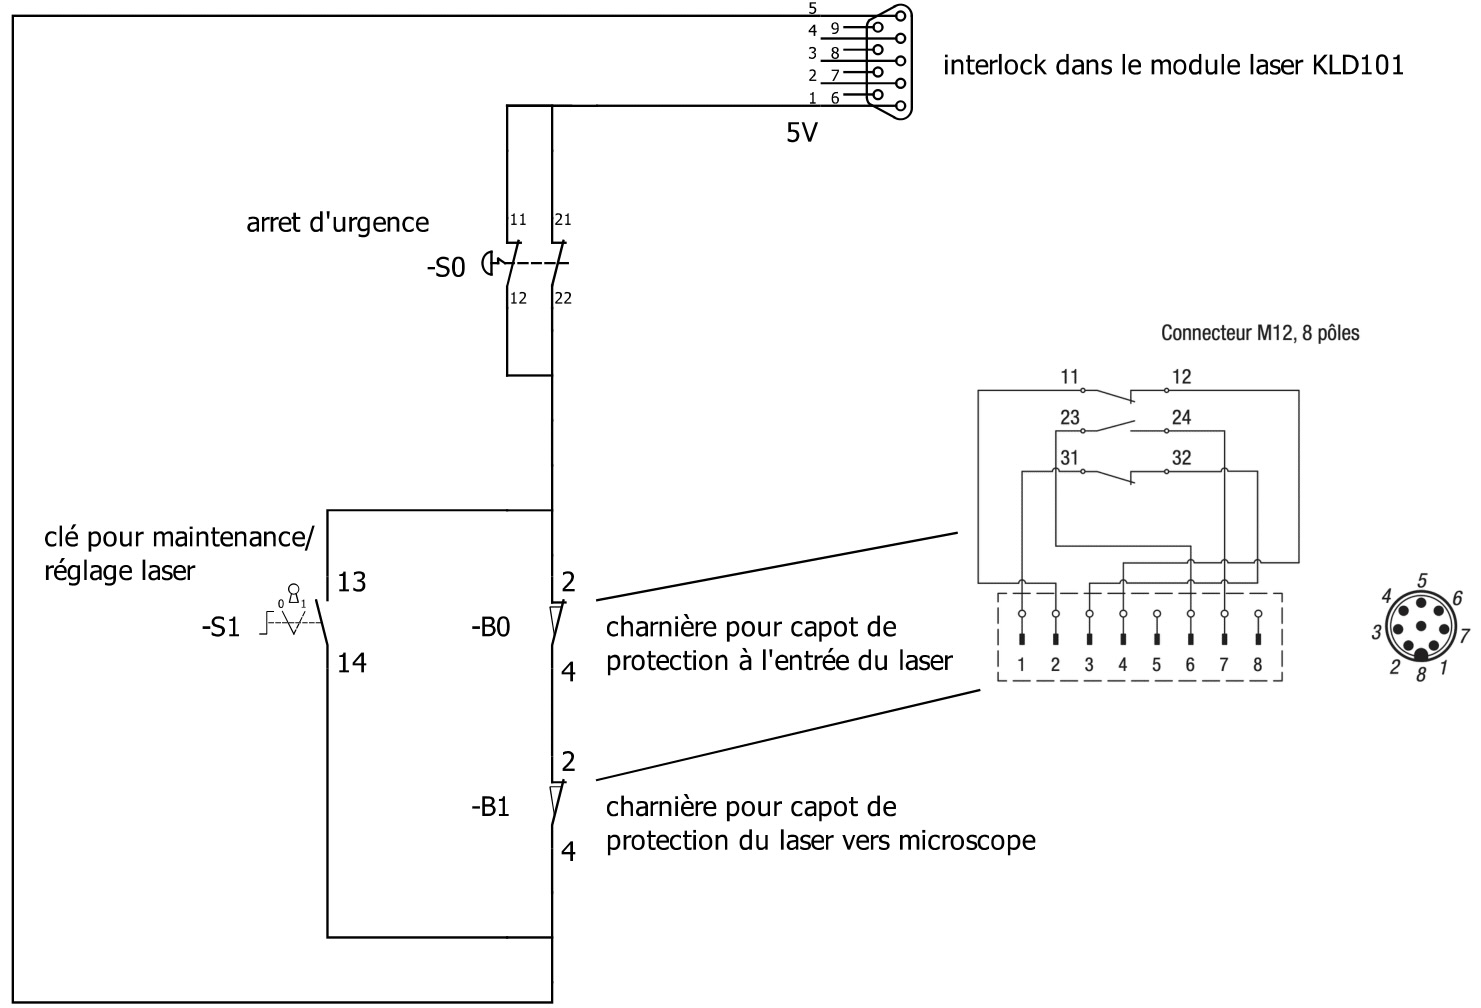
\includegraphics[width=\textwidth]{assets/figures/Protections_laser/interlock_schema_elec_V1.jpeg}
    \end{center}
    \caption{Première version du schéma électrique complet de l'interlock}
    \label{schema_interlock_v1}
\end{figure}
\newpage
\subsection{Capteurs sur les protections mécaniques}
Afin de garantir la sécurité lors de l'utilisation du laser, il est nécessaire de connaître quand une des deux protections est ouverte.

\subsubsection{Solutions disponibles sur le marché}
\begin{minipage}[c]{0.6\textwidth}
    Une première recherche s'est portée sur des interrupteurs de sécurité avec vérouillage électrique, que l'on retrouve beaucoup dans l'industrie. Ci-contre, un exemple de ce type d'interrupteur, voir Figure~\ref{interrupteur_telemecanique}.

    Ces serrures ont l'avantage qu'elles peuvent être vérouillées électriquement, ce qui permet d'assurer un vérouillage mécanique. Malheureusement, ce type de sécurité est trop volumineux pour notre système.
\end{minipage}\hfill
\begin{minipage}[c]{0.35\textwidth}
    \begin{center}
        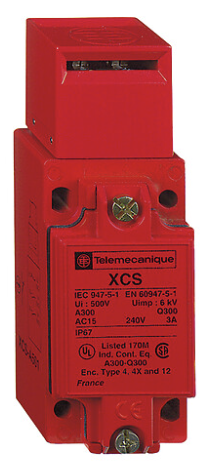
\includegraphics[width=0.45\textwidth]{assets/figures/Protections_laser/serrure_telemecanique.png}
    \end{center}
    \captionof{figure}{Interrupteur de sécurité Telemecanique~\cite{interrupteurTelemecanique}}
    \label{interrupteur_telemecanique}
\end{minipage}

\begin{minipage}[c]{0.6\textwidth}
    Une solution, chez le constructeur d'organes de sécurité Pilz, est une charnière comprenant un capteur intégré où l'on peut régler librement le point de commutation du contact entre 0\textdegree{} et 270\textdegree{}.

    Une photo ci-contre montre ce type de charnière électrique, voir Figure~\ref{charniere_pilz}.
\end{minipage}\hfill
\begin{minipage}[c]{0.35\textwidth}
    \begin{center}
        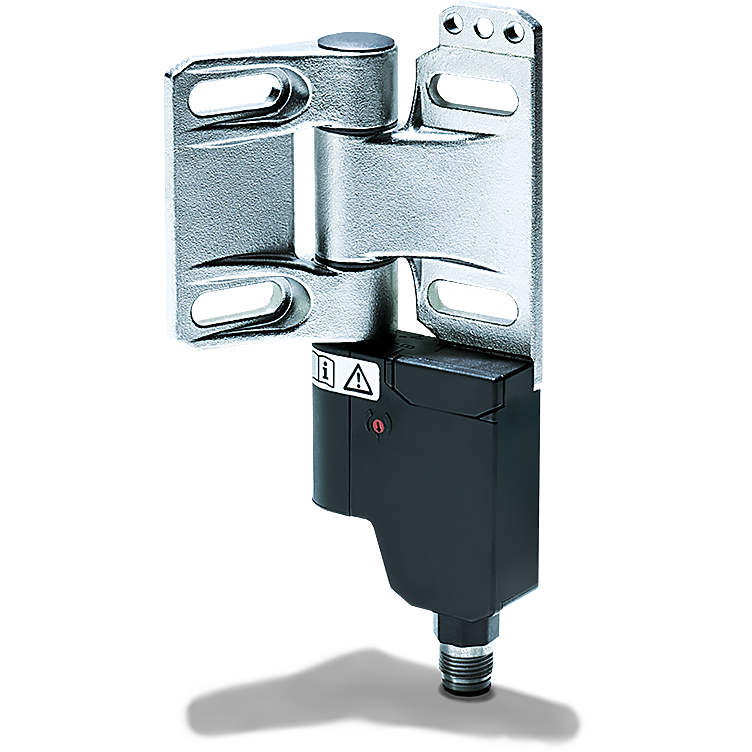
\includegraphics[width=0.6\textwidth]{assets/figures/Protections_laser/charniere_pilz.png}
    \end{center}
    \captionof{figure}{Charnière de sécurité Pilz~\cite{charnierePilz}}
    \label{charniere_pilz}
\end{minipage}

\begin{minipage}[c]{0.6\textwidth}
    Une dernière solution de charnière de sécurité a été élaborée par l'entreprise Norelem. Avec cette charnière, on peut également régler l'angle de commutation. L'avantage avec cette charnière est que le capteur est directement intégré dans la charnière, le rendant totalement invisible.

    Ci-contre, une photo de la charnière de Norelem, voir Figure~\ref{charniere_norelem}.
\end{minipage}\hfill
\begin{minipage}[c]{0.35\textwidth}
    \begin{center}
        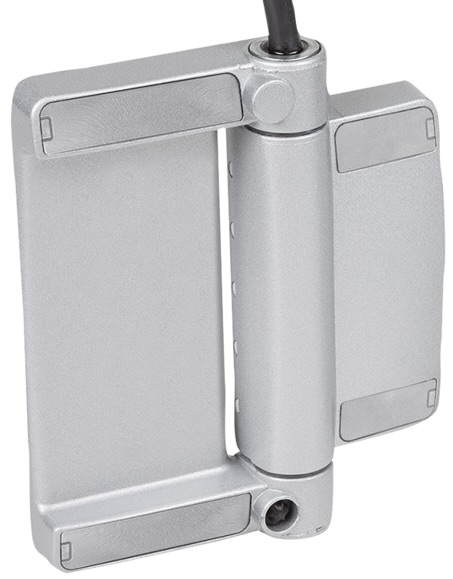
\includegraphics[width=0.75\textwidth]{assets/figures/Protections_laser/charniere_norelem.jpeg}
    \end{center}
    \captionof{figure}{Charnière de sécurité Norelem~\cite{charniereNorelem}}
    \label{charniere_norelem}
\end{minipage}

\begin{minipage}[c]{0.6\textwidth}
    Le fin de course est beaucoup utilisé en électronique car ne prends pas beaucoup de place et est facile à implémenter. Bien que cette solution soit discrète, cela reste un système de sécurité simple, et peut être facilement contourné.

    Ci-contre, une photo du fin de course, voir Figure~\ref{fin_de_course}.
\end{minipage}\hfill
\begin{minipage}[c]{0.35\textwidth}
    \begin{center}
        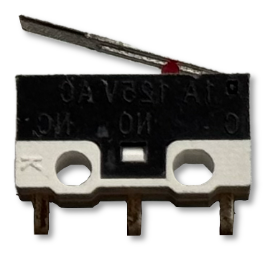
\includegraphics[width=0.6\textwidth]{assets/figures/Protections_laser/fin_de_course.png}
    \end{center}
    \captionof{figure}{Fin de course}
    \label{fin_de_course}
\end{minipage}

\newpage
\subsubsection{Solution choisie pour la protection à l'entrée du laser}
La solution finale pour cette protection s'est tournée sur la charnière de sécurité de l'entreprise Norelem. Elle contient tous les avantages que l'on recherche pour ce travail :
\begin{itemize}
    \item Elle s'intègre dans la conception de la protection, car on a de toute façon besoin d'une charnière pour soulever la protection.
    \item Elle contient un capteur de position intégré.
    \item L'angle de commutation est réglable.
    \item Elle est compacte, ce qui facilite son intégration dans le kit actuel.
    \item Il s'agit d'une solution robuste, conçue pour un usage industriel, donc va durer dans le temps.
\end{itemize}

\subsubsection{Solution choisie pour la protection vers le microscope}
La solution finale pour cette protection s'est tournée sur le fin de course. Ses avantages :
\begin{itemize}
    \item Vu qu'il n'y a pas beaucoup de place vers le microscope pour faire une protection, sa taille permet d'être installer presque où on veut.
    \item Il est peu coûteux et facilement remplaçable.
    \item Malgré sa sécurité simple, des solutions existent pour cacher le fin de course afin qu'il ne soit pas accessible facilement.
\end{itemize}

\subsection{Boîtier de sécurité : arrêt d'urgence et clé de maintenance}
\label{subsec:arret_urgence_maintenance}
L'ajout d'un arrêt d'urgence est l'une des principales sécurité électrique que l'on retrouve sur tout type de système électrique. Comme indiqué sur le schéma électrique de la Figure~\ref{schema_interlock_v1}, l'arrêt d'urgence est en série de tout le circuit interlock, ce qui permet de couper l'alimentation du laser à tout moment en pressant dessus.

La clé de maintenance, comme indiqué sur le schéma électrique de la Figure~\ref{schema_interlock_v1}, est en parallèle des deux capteurs. Comme son nom l'indique, en enclenchant cette clé, elle permet de faire la maintenance. En effet, en position fermée, les deux capteurs n'ont plus d'influence sur l'ouverture du circuit interlock. Il peut arriver qu'il faille effectuer réglages sur les lentilles réglables ou sur le laser, et que le laser doive rester allumé même avec les protections ouvertes. Voir la Figure \ref{boitier_arret_urgence_maintenance}.

\begin{figure}[H]
    \begin{center}
        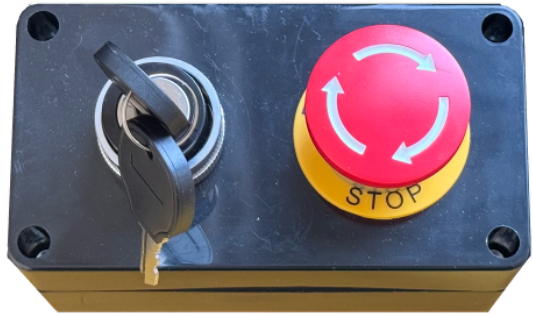
\includegraphics[width=0.7\textwidth]{assets/figures/Protections_laser/boitier_arret_urgence_maintenance.png}
    \end{center}
    \caption{Boitier comprenant l'arrêt d'urgence et la clé de maintenance}
    \label{boitier_arret_urgence_maintenance}
\end{figure}


\newpage
\section{Protection à l'entrée du laser}
\subsection{Exigences fonctionnelles de la protection}
Cette section a pour but de détailler les différentes exigences que la protection va devoir remplir.

La protection :
\begin{enumerate}
    \item assurera une protection complète contre les réflexions du laser, afin de garantir la sécurité des utilisateurs du kit.
    \item ne devra pas restreindre l'accessibilité des autres composants, tels que les lentilles réglables ainsi que le laser, afin de pouvoir régler ceux-ci facilement, si nécessaire.
    \item sera un assemblage mécanique simple à monter et à démonter.
    \item aura une conception simple, afin que sa fabrication soit la plus aisée possible.
    \item comprendra le moins de pièces et de visseries possible.
\end{enumerate}

% POUR LE CHAT:
% Je t'explique ce que j'ai fais dessus:
% J'ai d'abbord fait une premiere version rapide en carton pour connaitre l'idee générale, ensuite je suis passer sur fusion 360 pour modéliser une protection vu que j'avais modéliser le kit en entier. avant la modélisation, j'ai du chercher une charnière qui a un contact intégré. Enfaite, avant cette partie protection, j'ai déjà réfléchie quels type de